\chapter{Methodology}
The research consists of 7 main phases as shown in figure \ref{fig:Overall}:

\begin{figure}[h!]
    \centering
    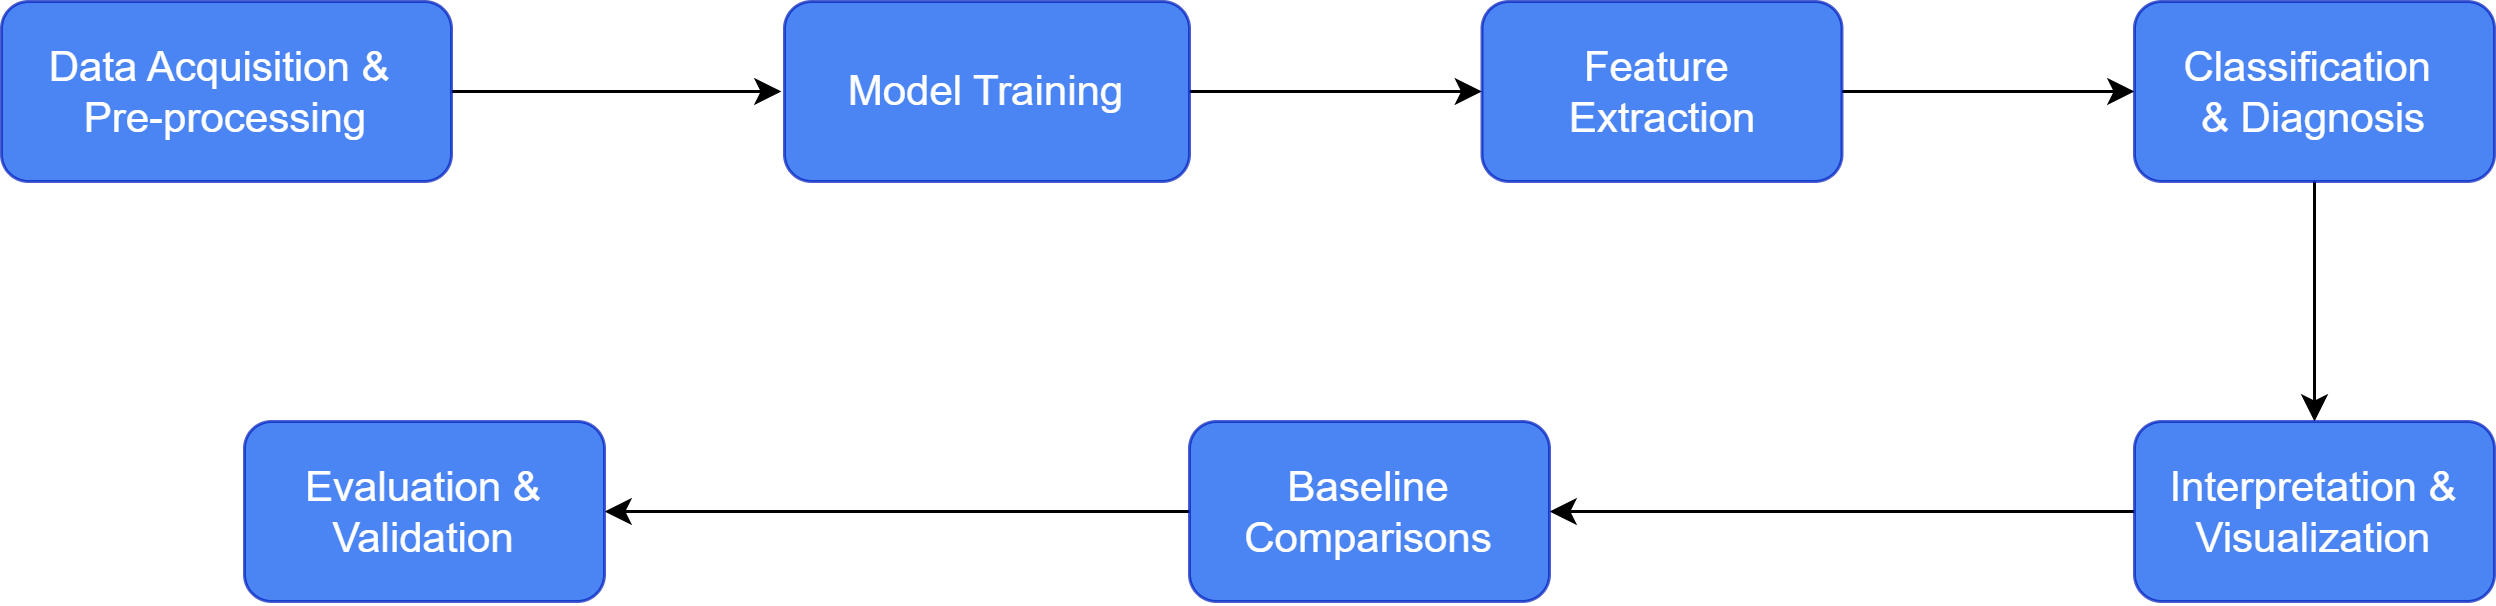
\includegraphics[width=0.95\textwidth]{overallpic.png}
    \caption{Overall Methodology}
    \label{fig:Overall}
\end{figure}

\section{Data acquisition and pre processing}
We selected two publicly available 3D chest CT datasets, CT-RATE\cite{ctrate} and ReXGroundingCT\cite{rexgroundingct}, for training and
evaluation due to their complementary nature. Their characteristics are summarized in table \ref{datasetTable}:


\begin{table}[ht]
    \centering
    \small
    \setlength{\tabcolsep}{6pt}
    \caption{Characteristics of CT-RATE and RexGroundingCT datasets}
    \label{datasetTable}

    \resizebox{\textwidth}{!}{%
    \begin{tabular}{|c|c|c|}
        \hline
        Feature & CT-RATE dataset & RexGroundingCT dataset \\
        \hline
        \makecell[c]{Type of Data}
            & \makecell[c]{3D non contrast chest CT volumes with \\ corresponding radiology text reports and \\ multi abnormality labels}
            & \makecell[c]{Subset of CT-RATE scans paired with free-text \\ findings and pixel level 3D segmentation masks} \\
        \hline
        \makecell[c]{Number of Scans}
            & \makecell[c]{25,692 non contrast chest CT studies \\ (50,188 volumes after reconstruction)}
            & \makecell[c]{3,142 non contrast chest CT scans} \\
        \hline
        \makecell[c]{Number of patients}
            & \makecell[c]{21,304 unique patients.}
            & \makecell[c]{Subset selected from CT-RATE} \\
        \hline
        \makecell[c]{Associated Reports}
            & \makecell[c]{Full radiology reports (findings and \\ impressions) with structured multi \\ abnormality labels (18 categories)}
            & \makecell[c]{Standardized radiology reports from \\ CT-RATE used to extract free text findings} \\
        \hline
        \makecell[c]{Annotations}
            & \makecell[c]{Text image pairs with structured labels; \\ no voxel wise ground truth segmentations}
            & \makecell[c]{Manual pixel level 3D segmentations \\ of findings extracted from reports \\ (8,028 findings; 16,301 entities)} \\
        \hline
    \end{tabular}%
    }
\end{table}

Data pre processing corrections such as intensity normalization and spacing adjustments have already been implemented directly in
the dataset. If further pre processing is required, standard techniques such as resampling to a uniform voxel size, intensity
normalization, and lung segmentation, shall be implemented before feeding the data into the model. Both datasets are released under MIT licenses that
allow use for non commercial academic research.

\section{Model Training}

\begin{figure}[!htbp]
    \centering
    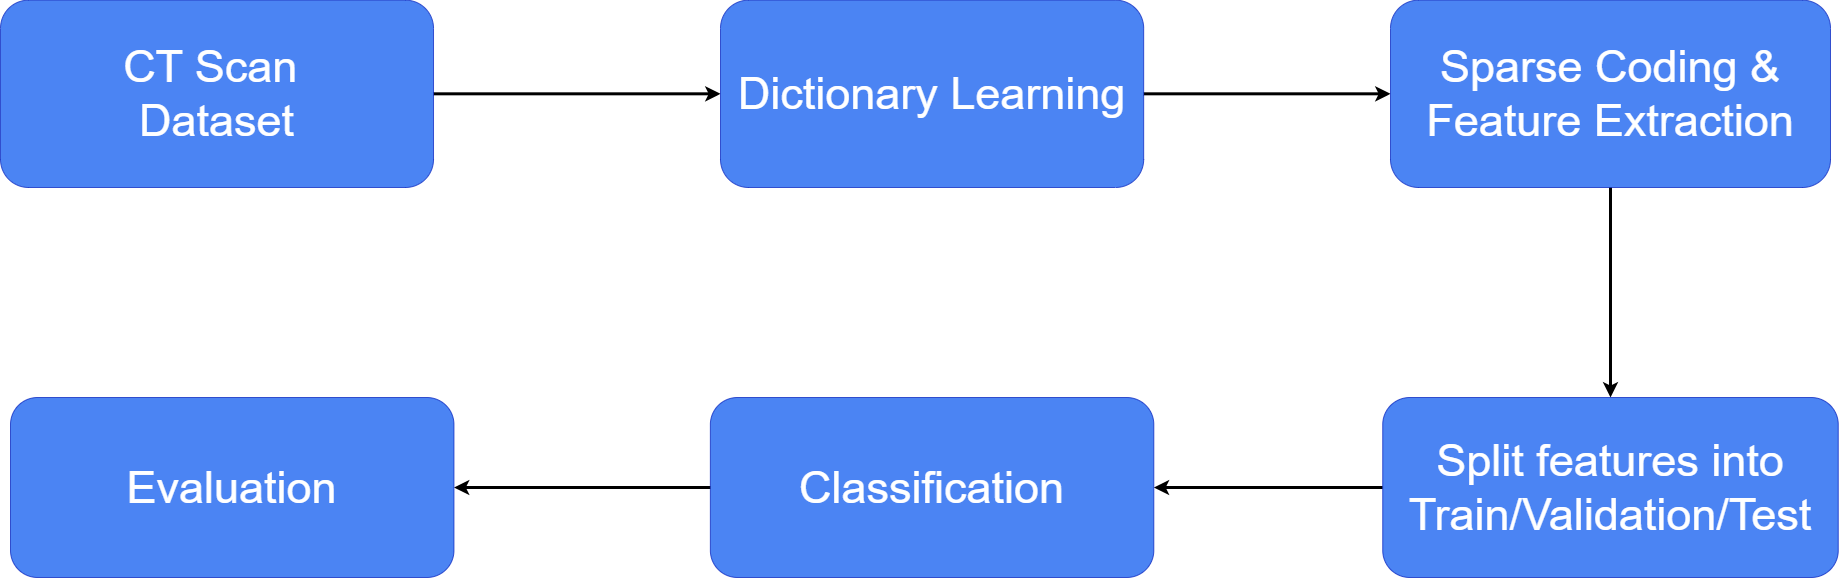
\includegraphics[width=0.7\textwidth,height=0.6\textheight,keepaspectratio]{ModelTraining.png}
    \caption{Model Training Workflow}
    \label{fig:Training}
\end{figure}

Model training will be implemented using a frozen dictionary learning approach to capture both normal and pathological
patterns in chest CT scans. The dataset will be divided into train, test and validation sets. The approach first learns a dictionary from
healthy lung scans to model normal anatomical patterns. Then, while keeping this normal representation fixed, incrementally learns
additional atoms to capture disease specific pathological features during sparse coding.

We extend the dictionary learning approach using \ac{LCKSVD} to improve the discriminative power of the learned sparse representations.
The label consistency constraint will produce similar sparse codes for CT samples belonging to the same disease category. \ac{LCKSVD}
will be formulated to jointly optimize three key objectives:
\begin{enumerate}
    \item Accurate reconstruction of CT image patches using the learned dictionary.
    \item Consistency of sparse representations within the same disease class.
    \item Effective classification of lung conditions based on the sparse codes.
\end{enumerate}
Appropriate weighting will be applied to balance these objectives and hyperparameters will be selected through validation experiments.

\section{Classification and Disease Diagnosis}

Disease classification will be performed using a low order linear classifier operating on the sparse representations produced by the
learned dictionary. In particular, classification is achieved by applying a linear projection to the sparse codes, followed by a
softmax based decision rule. This approach enables multi class prediction while maintaining a small number of trainable parameters.
The classification module will be implemented in Python using scikit learn.

Diagnostic Hypotheses will be done for the following 10 disease classes:
\begin{enumerate}
    \item COPD or Emphysema
    \item Heart Failure or Cardiomyopathy
    \item Pericarditis
    \item Atherosclerotic Cardiovascular Disease
    \item Pneumonia (Viral, bacterial, Tuberculosis, COVID-19)
    \item Bronchiectasis
    \item Lung Cancer (Primary or Metastatic)
    \item Lymphoma or Sarcoidosis
    \item Hiatal Hernia
    \item Pulmonary Embolism
\end{enumerate}

\section{Interpretability Analysis and Visualization}
To improve interpretability and clinical relevance, the learned dictionary atoms will be visualized and analyzed through an interactive
user interface utilizing 3D rendering techniques. Each dictionary atom will be mapped back to the original CT image space, allowing us
to see which anatomical regions or pathological patterns the model has learned to represent. This mapping is guided by the ReXGroundingCT
annotations, which provide precise spatial localization of abnormalities within the 3D imaging volume.Interpretability is measured using 
semantic coherence, atom to pattern correspondence, reconstruction fidelity, and segmentation accuracy, which together evaluate how 
meaningfully each learned atom represents clinically relevant structures when mapped back to the original 3D CT space.

\section{Volumetric Feature Extraction and Quantification}
Volumetric quantification of pulmonary patterns will be performed using segmentation to differentiate between the 18 radiological abnormalities
defined in the CT-RATE dataset. Particular focus will be placed on quantifying consolidation and ground-glass opacities (GGO), as these patterns
are critical indicators of disease severity in various pulmonary conditions. Using the segmentation masks provided in the ReXGroundingCT dataset,
the total volumes of consolidation and GGO will be calculated for each CT scan.
The C/G ratio will be computed by dividing the total volume of consolidation by the total volume of GGO across the entire lung parenchyma.
This quantitative metric provides an objective measure of disease severity and progression, with higher ratios indicating more
advanced pathological states. The calculated C/G ratios will be compared against model predictions and clinical thresholds to validate
the diagnostic utility of the learned dictionary representations. These volumetric features will complement the sparse coding analysis,
enabling a more comprehensive evaluation of the model's ability to capture clinically relevant patterns.

\section{Baseline Comparisons and Benchmarking}
The proposed method will be compared against well established baseline approaches commonly used in medical imaging research. These
baselines are chosen to represent both traditional machine learning techniques and modern deep learning models. Standard K-SVD is
included as a baseline to highlight the advantage of incorporating label information through LC-KSVD. By comparing these two
sparse representation methods, the contribution of label consistent dictionary learning to disease classification performance can be
assessed.

In addition, several 3D CNN architectures will be used as deep learning baselines,
as they are considered state of the art for volumetric CT analysis\cite{Tiwari2023Comprehensive}. 
These models are capable of learning complex spatial patterns across multiple slices and therefore provide a strong benchmark against
which the proposed method can be evaluated. Existing implementations of these networks will be adopted to ensure reliability and consistency.
All models will be trained and tested using the same dataset, although training strategies may differ due to the higher data and computational
demands of CNN-based approaches.

All methods will be implemented using suitable and widely adopted frameworks, including scikit-learn for classical machine learning
and sparse coding methods, and PyTorch or TensorFlow for deep learning based models.

\section{Evaluation Metrics and Validation Strategy}
The performance of the proposed model will be evaluated using accuracy, precision, recall, F1-score, and AUC-ROC, which are standard
and widely accepted metrics in medical image analysis. Greater emphasis will be placed on accuracy and recall, as they are especially
important in a clinical context to ensure overall reliability and to minimize missed disease cases, while the remaining metrics
provide additional insight into class wise performance and discriminative ability.